\documentclass{article}
\usepackage[utf8]{inputenc}
\usepackage{xcolor}
\usepackage{siunitx}
\usepackage{amsmath}
\usepackage{float}
\usepackage{graphicx}
\usepackage[italian]{babel}
\usepackage[normalem]{ulem}
\usepackage{circuitikz}

\ctikzset{voltage/bump b/.initial=0}

\renewcommand*\contentsname{Indice}

\title{Caratterizzazione di filtri RC passa-alto e passa-basso}
\author{Simone Aronica, Giovanni Bloise, \\
Gabriele Camisa, Giuseppe Casale}

\begin{document}

\maketitle
\tableofcontents
\pagebreak

\section{TODO}
\begin{itemize}
  \item coddio, ricontrolla le incertezze sulla frequenza di taglio, guarda che il passa alto non ha due cosi in parallelo! rimane uguale l'incertezza!
  \item CODDIO ABBIAMO PRESO LE MISURE CON L'INTERRUTTORE CHIUSO NEL PASSA BASSO... DOVEVAMO ESCLUDERLO... ALMENO CREDO... DIO CANE
  \item gli strumenti! [+ vanno anche i cavi negli strumenti?]
  \item ma vogliamo tabulare anche le incertezze della funzione di trasferimento in dB (quelle asimmetriche, secondo me non serve)?
  \item le conclusioni (cioè boooom guarda abbiamo l'attenuazione di almeno -3 dB sulla frequenza di taglio, cioè, spaziale ****)
  \item vanno fatti i diagrammi di bode asintotici? volendo si può eh, tanto dobbiamo farli comunque per il lab4, boh nsomma vedi un po'
  \item \sout{guarda che nelle tabelle voleva gradi per la differenza di fase, non tempi}
  \item \sout{controlla la formula per calcolare i gradi.} (ora dovrebbe andare), credo.
  \item \sout{andava plottato il modulo della funzione di trasferimento in teoria, non il modulo e basta.} il volere divino si è compiuto, alleluia, alleluia.
  \item \sout{ora mancano sicuro le immagini.} più che altro, controllale, ma dovrebbero essere ok.
  \item fatti, please, un diagramma asintotico a mano, metti che stai cannando qualcosa.
  \item \sout{ma è normale che in logaritmico ci sia più incertezza in negativo che in positivo nel passa alto?} (si, esce così)
\end{itemize}

\section{Strumenti usati}
\begin{itemize}
    \item Multimetro HP 34401A
    \item Rigol DS1054-Z
    \item Generatore di funzioni
\end{itemize}


\section{Sintesi dell'esperienza}

In questa esperienza di laboratorio è stato osservato il comportamento in frequenza di un circuito stampato che implementa un filtro RC passa-basso e passa-alto.

Come valutazione preliminare è stata verificata la compatibilità del valore effettivo della resistenza integrata nel circuito rispetto a quello nominale dichiarato dal produttore.
È stato trovato che questo valore è di $1021\pm11.2\ \SI{}{\ohm}$, che è compatibile con il valore dichiarato di $1000\pm800\ \SI{}{\ohm}$.
I condensatori sono stati considerati, come dichiarato dal produttore, di capacità $C=\SI{10}{\nano\farad}, 20\%$.

Dunque è stato impostato un generatore di segnali alla frequenza di $\SI{100}{\hertz}$ per generare un segnale sinusoidale di tensione picco-picco $\SI{800}{\milli\volt}$.\\
Tutte le misurazioni sono state effettuate tramite un oscilloscopio, tenendo il coefficiente di sensibilità verticale a $100\frac{\SI{}{\milli\volt}}{\text{div}}$.\\
Per il campionamento della risposta in frequenza del segnale d'ingresso è stato variato da $\SI{200}{\hertz}$ a $\SI{1}{\mega\hertz}$.

\section{Filtro passa-basso}
\begin{center}
\begin{circuitikz}
	\draw (0,0) to[short, *-*] (7,0)
	(3,0) to[C=$\SI{10}{\nano\farad}$, -] (3,2)
	(5,0) to[C=$\SI{10}{\nano\farad}$, -] (5,2)
	(0,2) to[R=$\SI{1}{\kilo\ohm}$, *-] (3,2)
	(3,2) -- (7,2)
	(0,0) to[open, v=$V_{\text{in}}$] (0,2)
	(7,0) to[open, v=$V_{\text{out}}$] (7,2)
	to[short, -*] (7,2);
\end{circuitikz}
\end{center}

\subsection{Frequenza di taglio}
La frequenza di taglio del filtro passa-basso è pari a:
\begin{equation*}
	f_{T}=\frac{1}{2\pi RC}=\frac{1}{2\pi\cdot\SI{1021}{\ohm}\cdot\SI{20}{\nano\farad}}=\SI{8.0}{\kilo\hertz}
\end{equation*}
con un'incertezza pari a:
\begin{equation*}
	\epsilon f_{T}=\epsilon R+\epsilon C = 5\%+40\% = 45\% \Rightarrow\delta f_T = \SI{3.6}{\kilo\hertz}
\end{equation*}

\subsection{Campionamento della risposta in frequenza}

\begin{table}[H]
	\makebox[\linewidth][c]{
		\begin{tabular}{|c|c|c|c|c|}
      % heading
      \hline
			$\text{Freq.\ /\SI{}{\hertz}}$ &
			$V_{\text{in}}\pm\delta V_{\text{in}}\ /\SI{}{\milli\volt}$ &
      $V_{\text{out}}\pm\delta V_{\text{out}}\ /\SI{}{\milli\volt}$ &
			$\Delta\phi\pm\delta(\Delta\phi)\ /\SI{}{\degree}$ &
			$20\log_{10}{(V_{\text{out}} / V_{\text{in}})}\ /\SI{}{\dB}$\\
      \hline
      %%% .1
			100 & $880\pm 80$ & $800\pm80$ & $0.0\pm1.44$ & -0.83\\
			\hline
			300 & $880\pm 80$ & $800\pm80$ & $0.0\pm4.32$ & -0.83\\
			\hline
			500 & $880\pm 80$ & $800\pm80$ & $0.0\pm7.2$ & -0.83\\
			\hline
			1k & $880\pm 80$ & $800\pm80$ & $3.6\pm7.2$ & -0.83\\
			\hline
			3k & $880\pm 80$ & $800\pm80$ & $8.64\pm8.64$ & -0.83\\
			\hline
			5k & $880\pm 80$ & $800\pm80$ & $18.0\pm3.6$ & -0.83\\
			\hline
			10k & $880\pm 80$ & $680\pm80$ & $29.52\pm1.44$ & -2.24\\
			\hline
			30k & $880\pm 80$ & $400\pm80$ & $62.64\pm4.32$ & -6.85\\
			\hline
			50k & $880\pm 80$ & $240\pm80$ & $72.0\pm3.6$ & -11.29\\
			\hline
			100k & $880\pm 80$ & $130\pm8$ & $79.2\pm7.2$ & -16.61\\
			\hline
			300k & $880\pm 80$ & $44\pm4$ & $95.04\pm4.32$ & -26.02\\
			\hline
			500k & $880\pm 80$ & $28\pm4$ & $93.6\pm7.2$ & -29.95\\
			\hline
			1M & $880\pm 80$ & $12\pm4$ & $90.0\pm14.4$ & -37.31\\
			\hline
		\end{tabular}
	}
	\caption{Misurazioni per filtro passa-basso}
\end{table}

\subsection{Diagrammi di Bode}

\begin{figure}[H]
  \makebox[\textwidth][c]{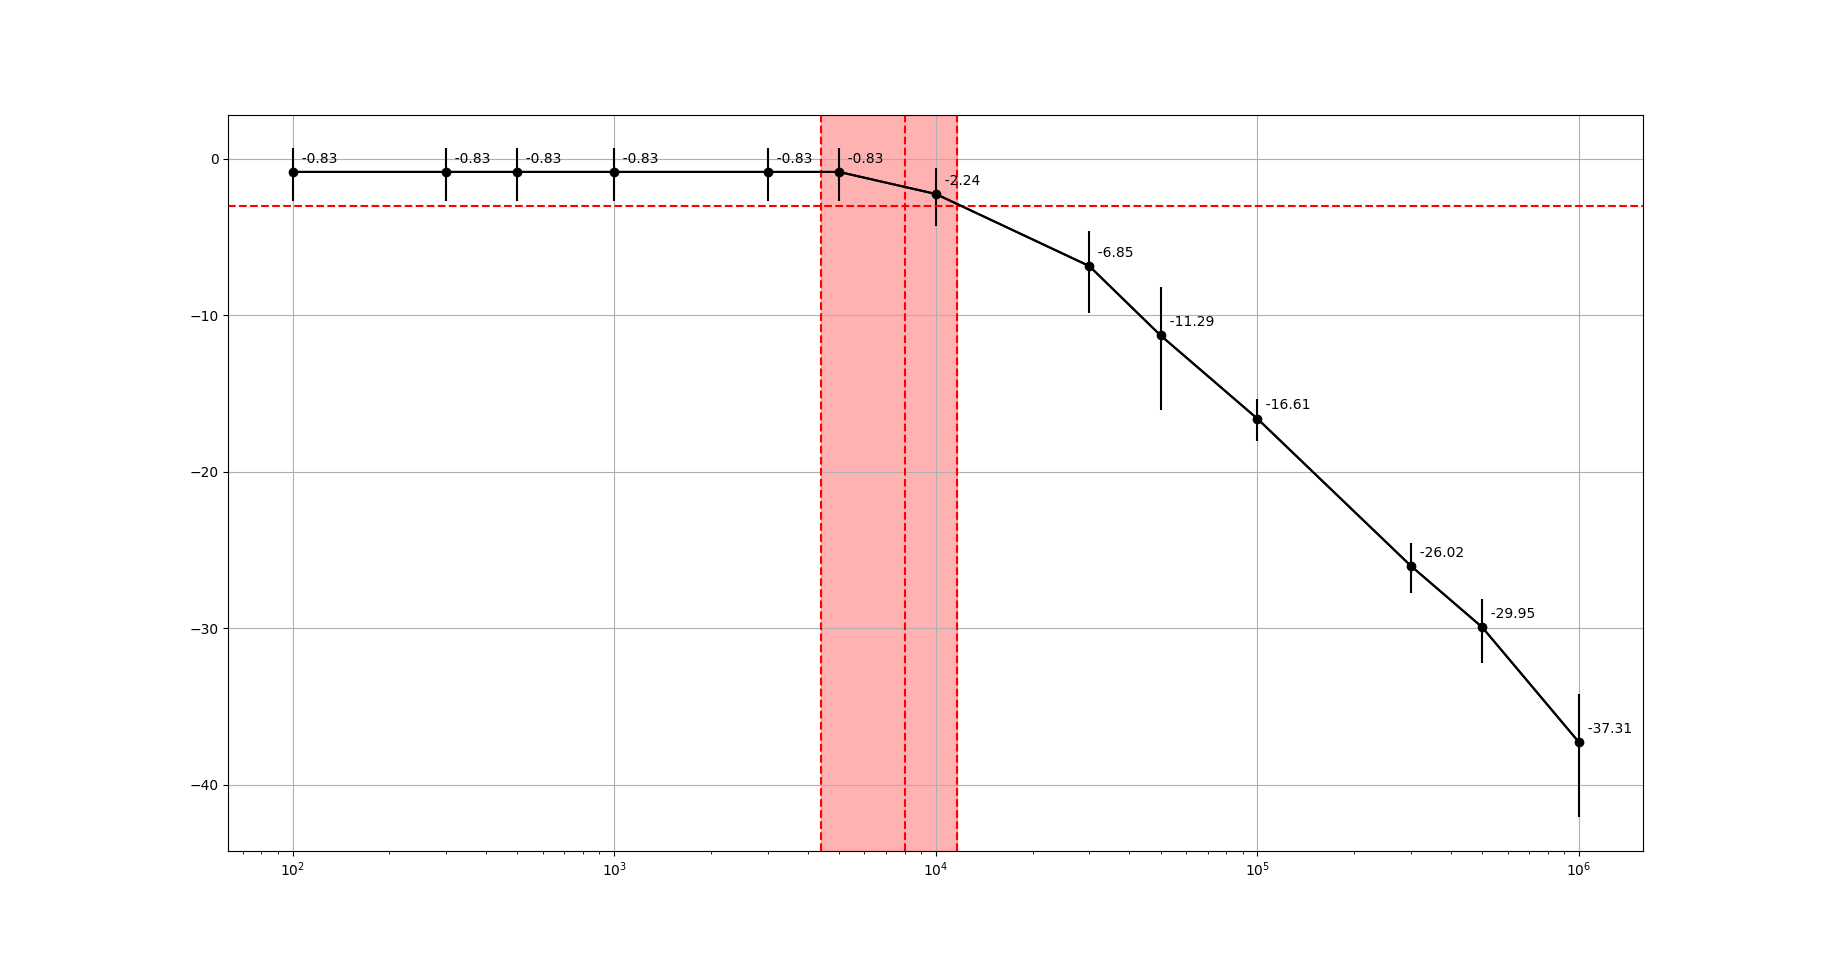
\includegraphics[width=2\linewidth]{img/PASSABASSOMODULO.png}}
  \caption{Diagramma di Bode del modulo per il filtro passa-basso}
\end{figure}
\begin{figure}[H]
  \makebox[\textwidth][c]{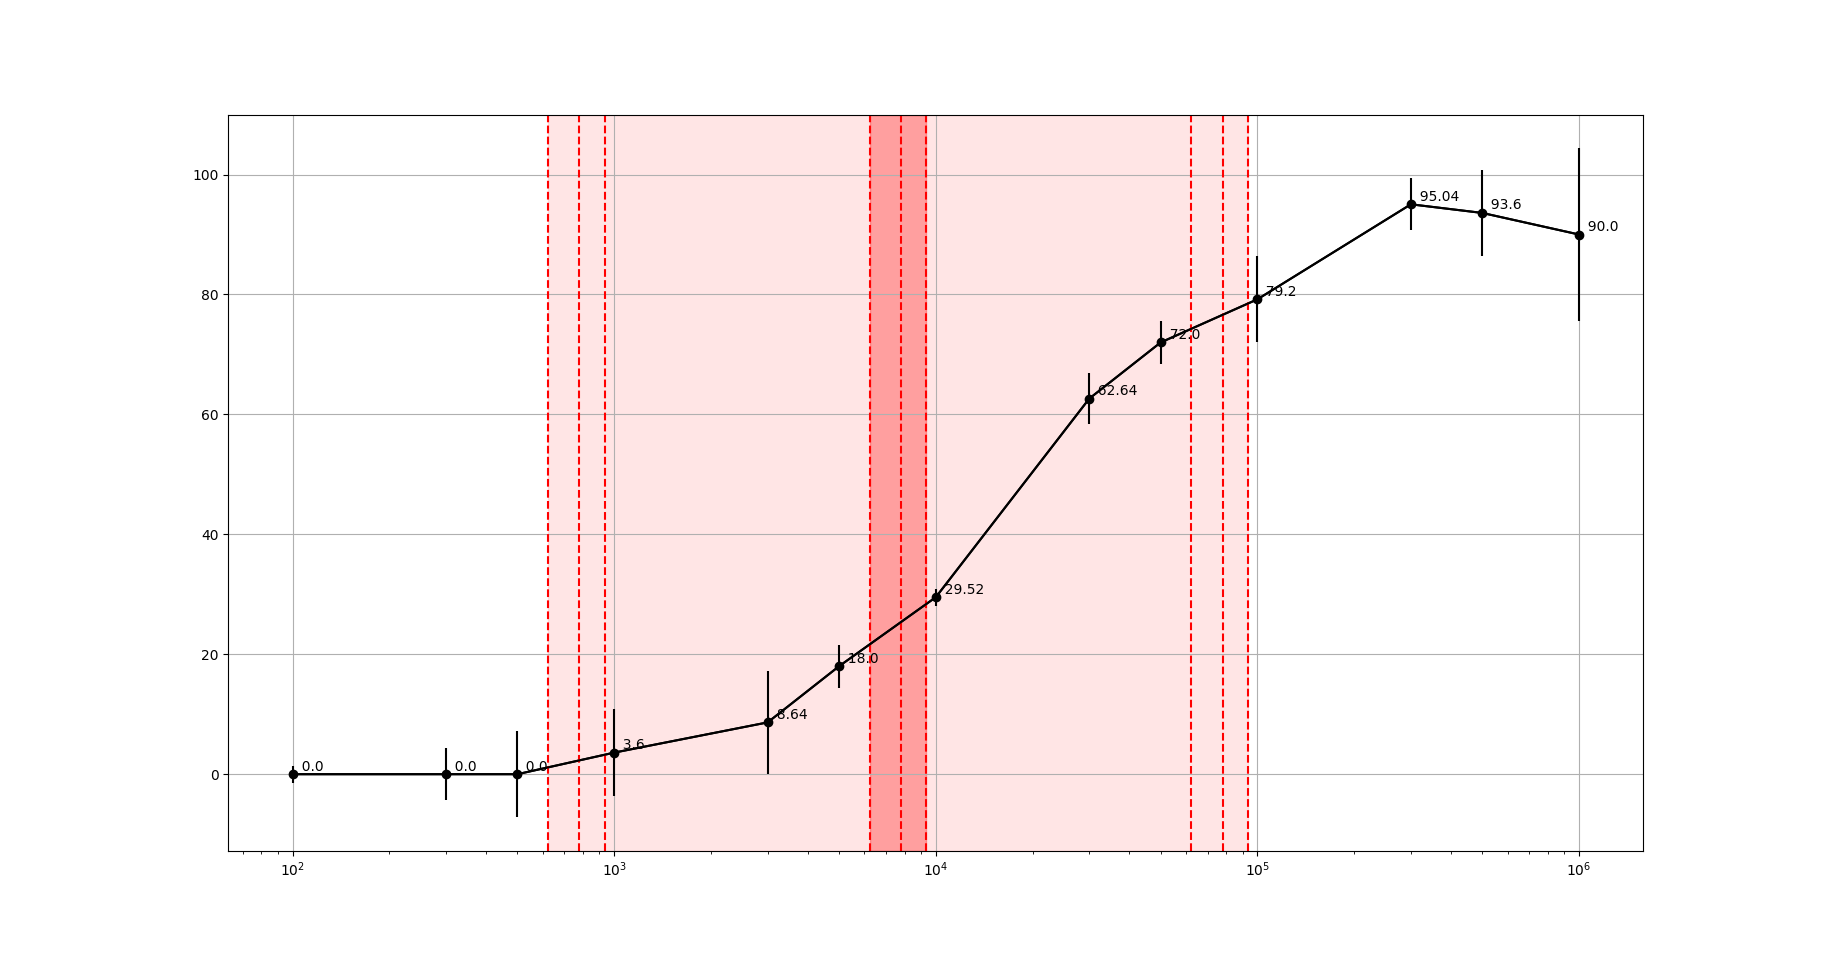
\includegraphics[width=2\linewidth]{img/PASSABASSOFASE.png}}
  \caption{Diagramma di Bode della fase per il filtro passa-basso}
\end{figure}

\section{Filtro passa-alto}

\begin{center}
\begin{circuitikz}
	\draw (0,0) to[short, *-*] (5,0)
	(3,0) to[R=$\SI{1}{\kilo\ohm}$, -] (3,2)
	(0,0) to[open, v=$V_{\text{in}}$] (0,2)
	(5,0) to[open, v=$V_{\text{out}}$] (5,2)
	(0,2) to[C=$\SI{10}{\nano\farad}$, *-] (3,2)
	to[short, -*] (5,2);
\end{circuitikz}
\end{center}


\subsection{Frequenza di taglio}
La frequenza di taglio del filtro passa-basso è pari a:
\begin{equation*}
	f_{T}=\frac{1}{2\pi RC}=\frac{1}{2\pi\cdot\SI{1021}{\ohm}\cdot\SI{10}{\nano\farad}}=\SI{16.0}{\kilo\hertz}
\end{equation*}
con un'incertezza pari a:
\begin{equation*}
	\epsilon f_{T}=\epsilon R+\epsilon C = 5\%+20\% = 25\% \Rightarrow\delta f_T = \SI{4.0}{\kilo\hertz}
\end{equation*}

\subsection{Campionamento della risposta in frequenza}

\begin{table}[H]
	\makebox[\textwidth][c]{
		\begin{tabular}{|c|c|c|c|c|}
      % heading
      \hline
			$\text{Freq.\ /\SI{}{\hertz}}$ &
			$V_{\text{in}}\pm\delta V_{\text{in}}\ /\SI{}{\milli\volt}$ &
      $V_{\text{out}}\pm\delta V_{\text{out}}\ /\SI{}{\milli\volt}$ &
			$\Delta\phi\pm\delta(\Delta\phi)\ /\SI{}{\degree}$ &
			$20\log_{10}{(V_{\text{out}} / V_{\text{in}})}\ /\SI{}{\dB}$\\
      \hline
      %%% 
      100 & $880\pm 80$ & $5\pm0.5$ & $93.6\pm18.0$ & -44.91\\
			\hline
			300 & $880\pm 80$ & $16\pm3$ & $86.4\pm10.8$ & -34.81\\
			\hline
			500 & $880\pm 80$ & $16\pm8$ & $45.0\pm18.0$ & -34.81\\
			\hline
			1k & $880\pm 80$ & $80\pm80$ & $90.0\pm9.0$ & -20.83\\
			\hline
			3k & $880\pm 80$ & $160\pm80$ & $86.4\pm4.32$ & -14.81\\
			\hline
			5k & $880\pm 80$ & $240\pm80$ & $72.0\pm7.2$ & -11.29\\
			\hline
			10k & $880\pm 80$ & $400\pm80$ & $57.6\pm3.6$ & -6.85\\
			\hline
			30k & $880\pm 80$ & $720\pm80$ & $27.0\pm2.16$ & -1.74\\
			\hline
			50k & $880\pm 80$ & $760\pm80$ & $18.0\pm3.6$ & -1.27\\
			\hline
			100k & $880\pm 80$ & $760\pm80$ & $9.0\pm3.6$ & -1.27\\
			\hline
			300k & $880\pm 80$ & $800\pm80$ & $4.32\pm4.32$ & -0.83\\
			\hline
			500k & $880\pm 80$ & $800\pm80$ & $0.0\pm3.6$ & -0.83\\
			\hline
			1M & $880\pm 80$ & $800\pm80$ & $0.0\pm7.2$ & -0.83\\
			\hline
		\end{tabular}
	}
	\caption{Misurazioni per filtro passa-alto}
\end{table}

\subsection{Diagrammi di Bode}

\begin{figure}[H]
  \makebox[\textwidth][c]{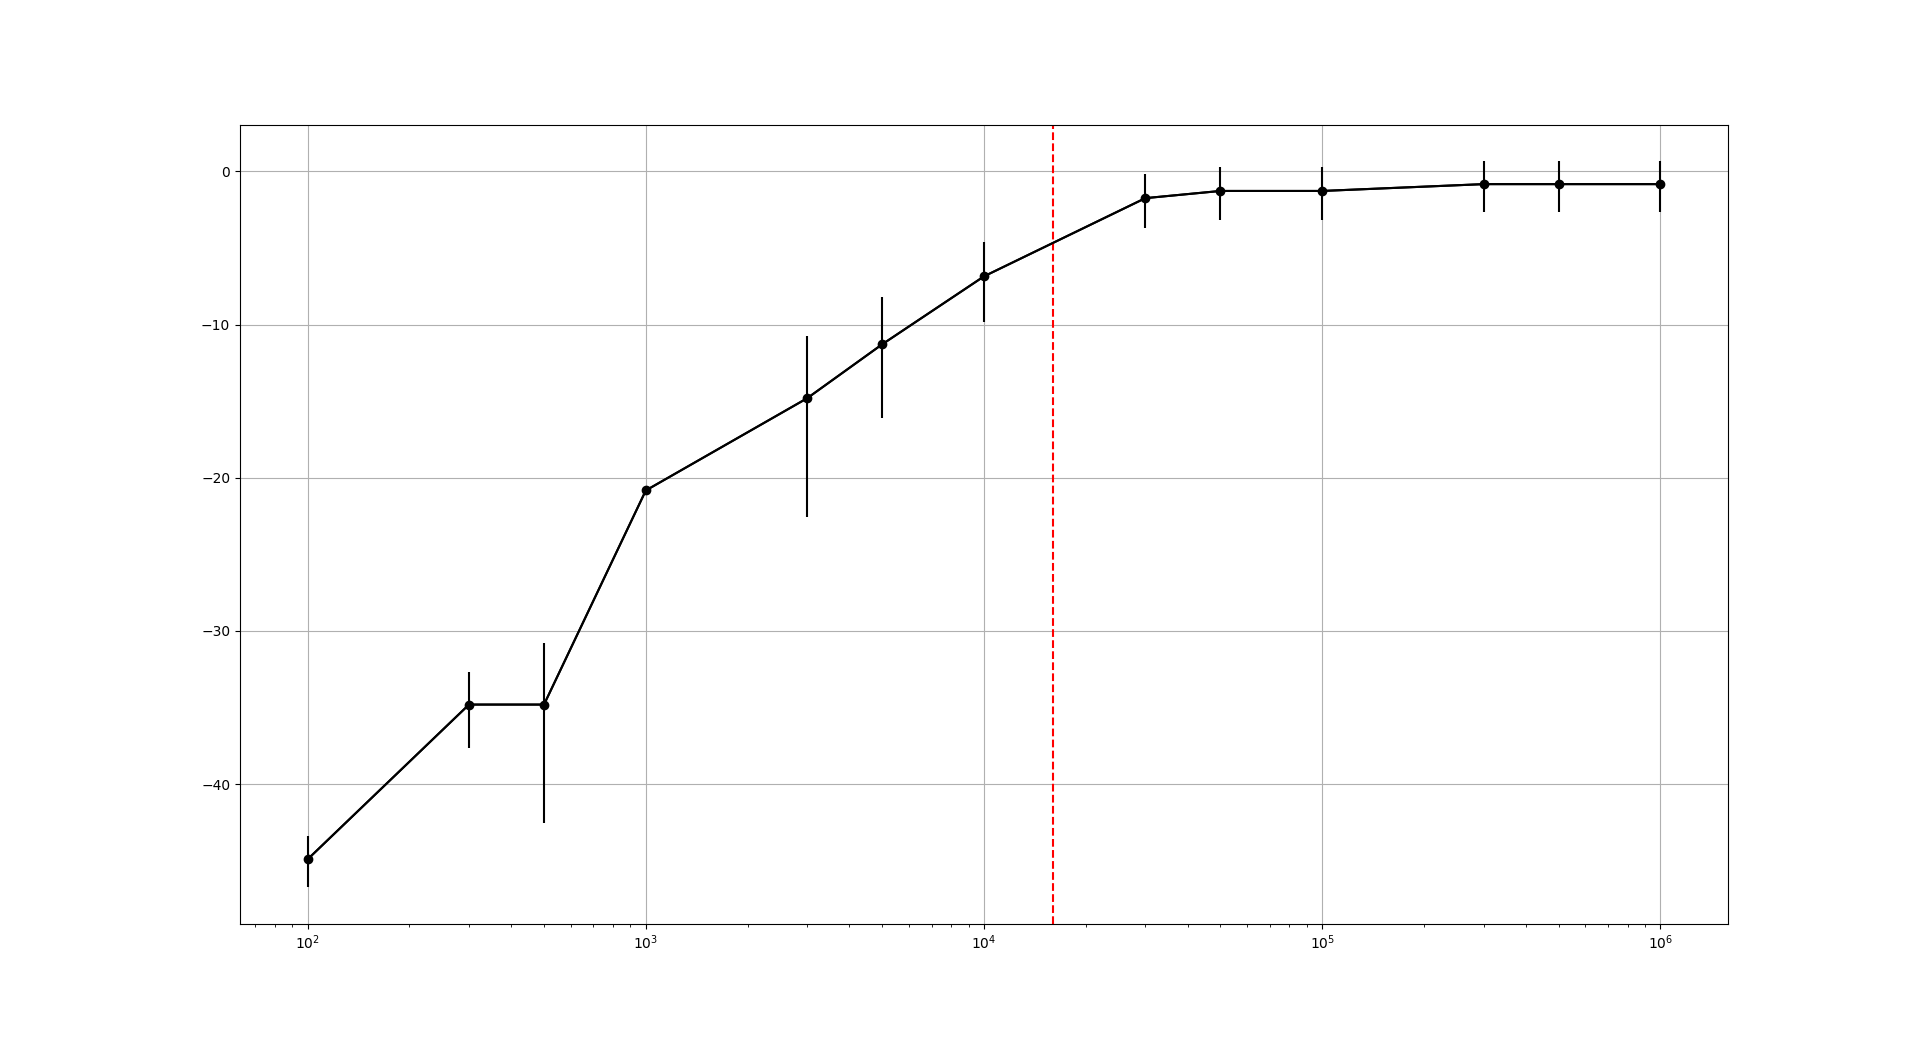
\includegraphics[width=2\linewidth]{img/PASSAALTOMODULO.png}}
  \caption{Diagramma di Bode del modulo per il filtro passa-alto}
\end{figure}
\begin{figure}[H]
  \makebox[\textwidth][c]{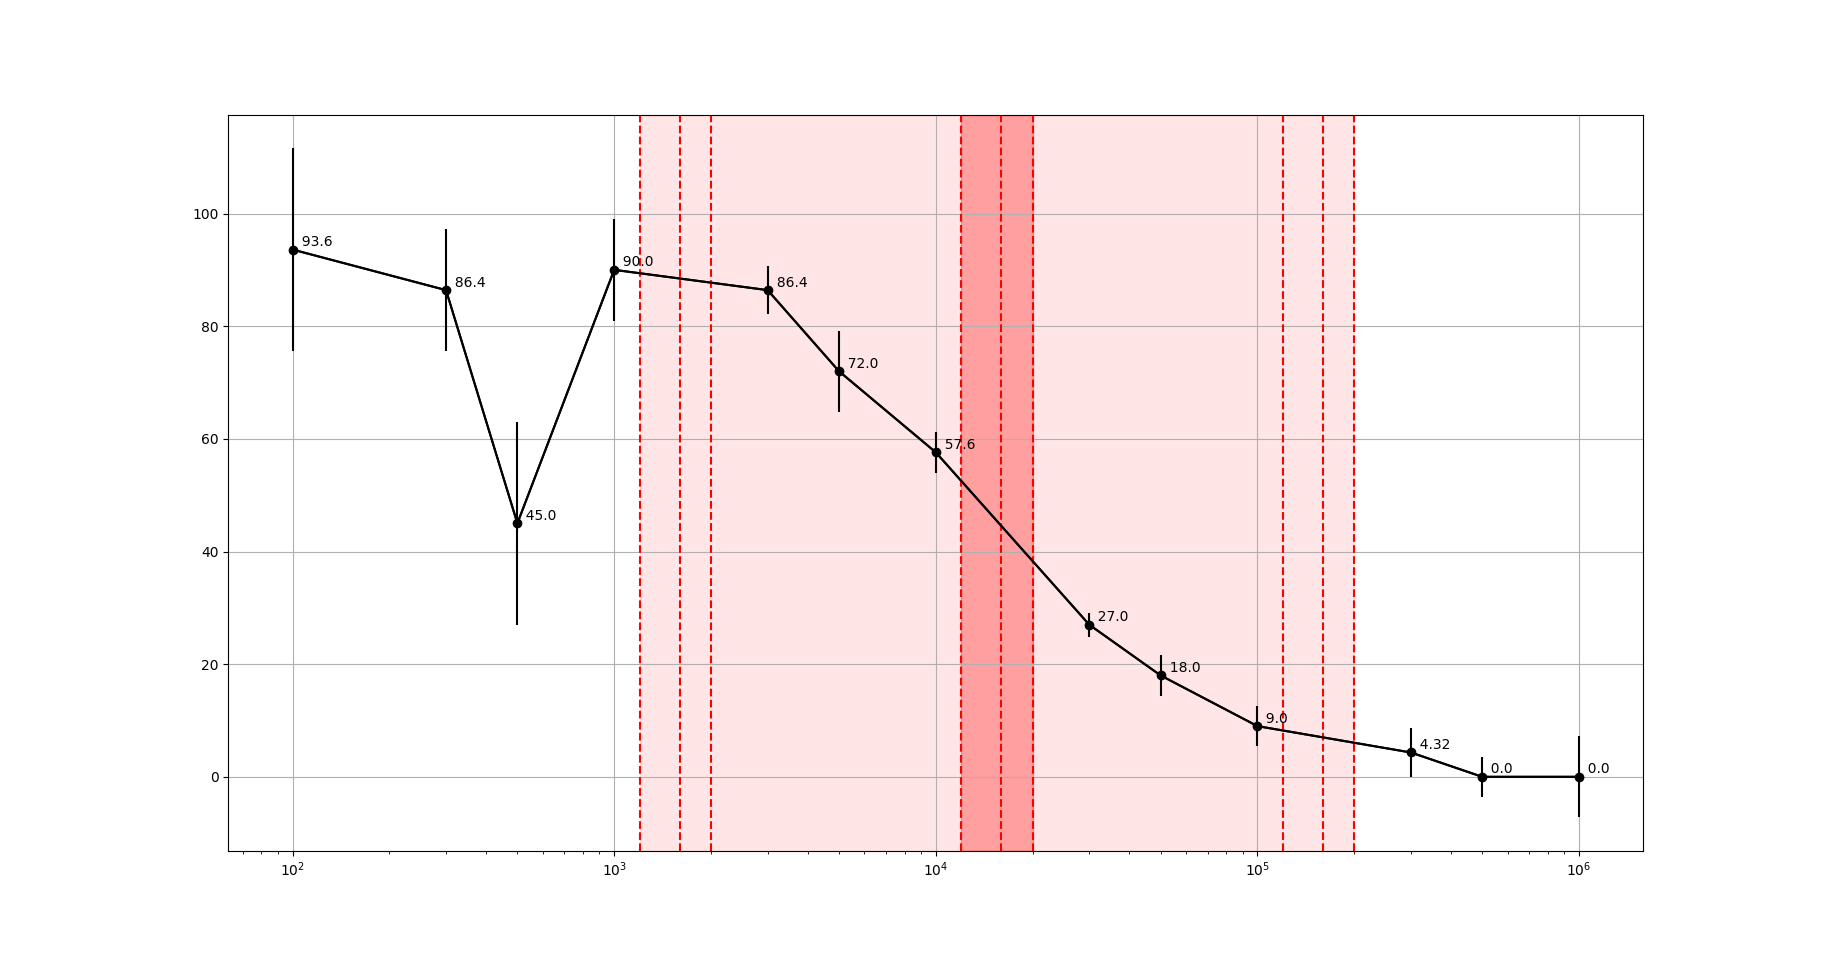
\includegraphics[width=2\linewidth]{img/PASSAALTOFASE.png}}
  \caption{Diagramma di Bode della fase per il filtro passa-alto}
\end{figure}

\section{Conclusioni}

\end{document}
